\chapter{Resultados y análisis}
\label{capitulo6}
\lhead{Capítulo 6. \emph{Resultados y análisis}}

\section{Pruebas en el EuRoC MAV Dataset}
A continuación se presentan los resultados obtenidos
utilizando las secuencias de datos  $MH\_ 01\_ easy$,  $MH\_ 05\_ difficult$,  $V1\_ 01\_ easy$,
$V1\_ 02\_ medium$ y  $V1\_ 03\_ difficult$, pertenecientes al EuRoC MAV Dataset.

En primera instancia se presentan los resultados directos del método iterativo de Gauss-Newton, y posteriormente los resultados obtenidos con la inicialización de este método utilizando los residuales de rotación provenientes del filtro inercial. Posteriormente se presentan los resultados obtenidos mediante el método RANSAC para la estimación del vector unitario de traslación.


\subsection{Evaluación del método de optimización de Gauss-Newton }

Para evaluar la estimación del método de Gauss-Newton se utilizó la secuencia $V1\_ 01\_ easy$ debido a que es una secuencia que presenta movimientos lentos y con mayor solapamiento entre imágenes, lo cual era un requisito para el método utilizado, ya que este utiliza un método directo para estimar la rotación y la traslación del robot. Los resultados de la orientación estimada de la cámara se presentan en la figura \ref{imagen:Resultados/GaussNewton/Orientacion}. En esta prueba se utilizó el detector SIFT y se utilizaron 4 escalas piramidales con un máximo número de iteraciones fijado a 10 para cada nivel. El tiempo promedio de estimación entre cada par de imágenes fue de 0.573243 s.

\begin{figure}[H]
	\centering
	\includegraphics[scale=0.6]{Resultados/GaussNewton/Orientacion}
	\caption{Orientación estimada de la cámara con el método de optimización de Gauss-Newton en secuencia $V1\_ 01\_ easy$. }
	\label{imagen:Resultados/GaussNewton/Orientacion}
\end{figure}

 La figura \ref{imagen:Resultados/GaussNewton/Posicion} muestra los resultados de la posición estimada, la cual se encuentra escalada con el desplazamiento real obtenido del groundtruth. 
 

\begin{figure}[H]
	\centering
	\includegraphics[scale=0.6]{Resultados/GaussNewton/Posicion}
	\caption{Posición estimada de la cámara con el método de optimización de Gauss-Newton en secuencia $V1\_ 01\_ easy$. }
	\label{imagen:Resultados/GaussNewton/Posicion}
\end{figure}

Con estos resultados es posible concluir que el método empleado diverge, ya que la orientación estimada no posee cambios, lo cual también se evidencia en la estimación de la posición de la cámara  en la figura \ref{imagen:Resultados/GaussNewton/Posicion}.

\subsubsection{Inicialización con residuales inerciales}
Debido a la divergencia del método de Gauss-Newton, se evaluaron nuevamente los resultados del método utilizando los residuales inerciales,  bajo la premisa de obtener estimaciones convergentes al inicializar el método en una estimación del movimiento rotacional más cercana a la real.

Los residuales inerciales y la orientación del robot provienen del filtro inercial. En la figura \ref{imagen:Resultados/GaussNewtonConResiduales1/ResidualOrientacionHistograma} se presentan los residuales inerciales utilizados en la inicialización. La figura \ref{imagen:Resultados/GaussNewtonConResiduales1/ErrorResidualOrientacion} muestra el error del residual y el error de orientación  se presenta en la figura \ref{imagen:Resultados/GaussNewtonConResiduales1/ErrorOrientacion}.

\begin{figure}[H]
	\centering
	\includegraphics[scale=0.6]{Resultados/GaussNewtonConResiduales1/ResidualOrientacionHistograma}
	\caption{ Residual de orientación estimado en secuencia $V1\_ 01\_ easy$.}
	\label{imagen:Resultados/GaussNewtonConResiduales1/ResidualOrientacionHistograma}
\end{figure}

\begin{figure}[H]
	\centering
	\includegraphics[scale=0.6]{Resultados/GaussNewtonConResiduales1/ErrorResidualOrientacion}
	\caption{ Error del residual de orientación estimado en secuencia $V1\_ 01\_ easy$.}
	\label{imagen:Resultados/GaussNewtonConResiduales1/ErrorResidualOrientacion}
\end{figure}

\begin{figure}[H]
	\centering
	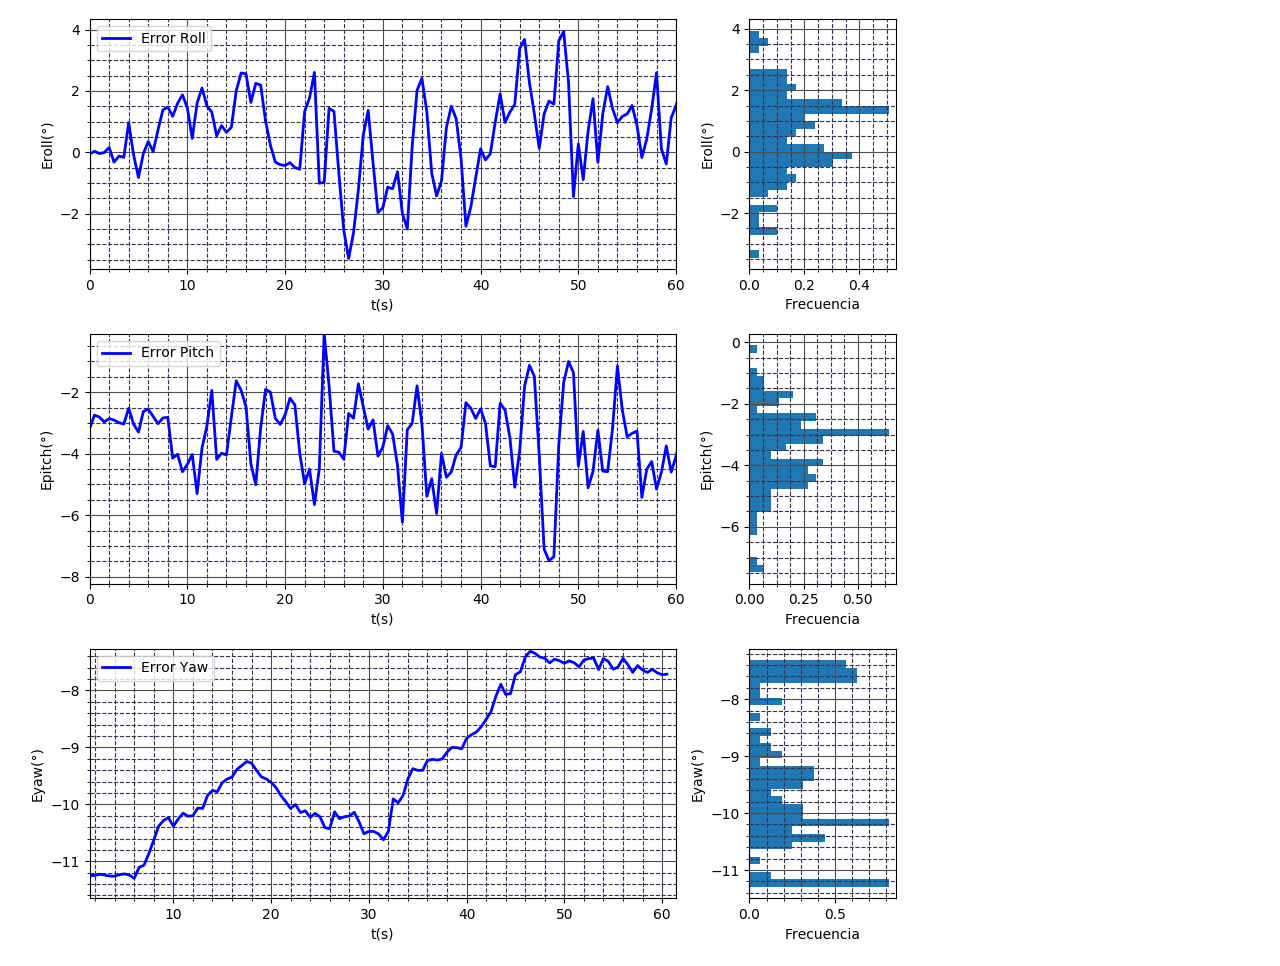
\includegraphics[scale=0.6]{Resultados/GaussNewtonConResiduales1/ErrorOrientacion}
	\caption{Posición estimada de la cámara con el método de optimización de Gauss-Newton en secuencia $V1\_ 01\_ easy$ empleando residuales inerciales. }
	\label{imagen:Resultados/GaussNewtonConResiduales1/ErrorOrientacion}
\end{figure}

Finalmente los resultados de la estimación de la posición se presentan en la figura \ref{imagen:Resultados/GaussNewtonConResiduales1/Posicion}.

\begin{figure}[H]
	\centering
	\includegraphics[scale=0.6]{Resultados/GaussNewtonConResiduales1/Posicion}
	\caption{Posición estimada de la cámara con el método de optimización de Gauss-Newton en secuencia $V1\_ 01\_ easy$ empleando residuales inerciales. }
	\label{imagen:Resultados/GaussNewtonConResiduales1/Posicion}
\end{figure}

En este caso la prueba realizada fue similar y se obtuvo un tiempo promedio de iteración del algoritmo de 0.799779 s, el cual es mayor al presentado sin la inicialización con residuales. En primer lugar esto indica que el algoritmo itera un mayor número de veces de la solución que minimice el error fotométrico. Es posible observar que la orientación de la cámara en este caso si es seguida debido a que el error de orientación se mantiene pequeño en los ángulos de roll y pitch, y sufre de drift en el angulo de yaw, lo cual se debe a que esta orientación es principalmente la orientación que se obtiene del filtro inercial. Sin embargo los resultados de la estimación de la posición no fueron satisfactorios.

También es posible observar en los histogramas de las figuras \ref{imagen:Resultados/GaussNewtonConResiduales1/ResidualOrientacionHistograma} y \ref{imagen:Resultados/GaussNewtonConResiduales1/ErrorResidualOrientacion} que el error porcentual del residual es relativamente alto para movimientos lentos, ya que en esta prueba la estimación de residuales se realiza imagen por imagen. Por estas razones, se realizó una segunda prueba calculando los residuales e inicializando el algoritmo de estimación cada 10 imágenes para comparar la estimación de la posición y el error de los residuales. En las figuras  \ref{imagen:Resultados/GaussNewtonConResiduales10/ResidualOrientacionHistograma}, \ref{imagen:Resultados/GaussNewtonConResiduales10/ErrorResidualOrientacion} y \ref{imagen:Resultados/GaussNewtonConResiduales10/Posicion} se muestran los resultados.

\begin{figure}[H]
	\centering
	\includegraphics[scale=0.6]{Resultados/GaussNewtonConResiduales10/ResidualOrientacionHistograma}
	\caption{ Residual de orientación estimado en secuencia $V1\_ 01\_ easy$.}
	\label{imagen:Resultados/GaussNewtonConResiduales10/ResidualOrientacionHistograma}
\end{figure}

\begin{figure}[H]
	\centering
	\includegraphics[scale=0.6]{Resultados/GaussNewtonConResiduales10/ErrorResidualOrientacion}
	\caption{ Error del residual de orientación estimado en secuencia $V1\_ 01\_ easy$.}
	\label{imagen:Resultados/GaussNewtonConResiduales10/ErrorResidualOrientacion}
\end{figure}


\begin{figure}[H]
	\centering
	\includegraphics[scale=0.6]{Resultados/GaussNewtonConResiduales10/Posicion}
	\caption{Posición estimada de la cámara con el método de optimización de Gauss-Newton en secuencia $V1\_ 01\_ easy$ empleando residuales inerciales. }
	\label{imagen:Resultados/GaussNewtonConResiduales10/Posicion}
\end{figure}

En esta prueba se tuvo un tiempo promedio de 0.739407 s y se puedo observar que el error porcentual de los residuales es más pequeño. Esto indicó que los residuales de orientación tendían a ser más exactos a mayores rangos de movimiento rotacional, lo cual los hace incompatibles con el método de optimización empleado ya que este requiere rangos mínimos de movimiento, lo cual se comprueba nuevamente con la divergencia de la estimación de la posición.

\subsection{Evaluación del método RANSAC}

En la evaluación del metodo de dos puntos se utilizaron secuencias lentas $MH\_ 01\_ easy$ y $V1\_ 01\_ easy$ y la secuencia rápida $V1\_ 02\_ medium$, para comparar el desempeño de los diferentes detectores ante cambios bruscos de movimiento. 

En este caso se utilizaron los detectores KAZE, AKAZE, ORB, SIFT y SURF en la evaluación. Las siguente secciones presentan los resultados de rendimiento de cada detector.

 Además se presentan las gráficas de posición, error de orientación y residuales de velocidad del detector con mejor estimación del conjunto y del detector con mejor eficiencia computacional. Esto, a manera de resumen debido a que la orientación y los residuales de velocidad en general son similares en cada detector empleado, ya que dependen en mayor medida del filtro inercial.  El conjunto total de gráficas de resultados para cada detector pueden ser visualizadas en la sección de resultados del  \href{https://github.com/Lujano/tesis/tree/master/imagenes/Resultados/}{\underline{repositorio del libro de tesis}}.
 
 
En cada sección se presentan los parámetros de configuración utilizados para la ejecución del sistema, como el umbral del RANSAC, el número de frames estáticos, el umbral para las disparidades euclidiana, rotacional y traslacional, y el umbral definido al detector utilizado. 
 
 El umbral del RANSAC representa el valor absoluto del máximo valor permisible del resultado del producto punto del vector de traslación estimado y el vector normal al plano epipolar de un punto característico, para ser clasificado como inlier. Es decir, si el valor absuluto del resultado es menor al umbral, el vector normal generado por la pareja de puntos característicos es clasificado dentro del modelo (inlier).
 
 La disparidad euclidiana es el promedio de distancia en unidades de píxeles de las parejas de puntos característicos en cada imagen. Un frame es considerado estático cuando no es keyframe y la disparidad euclidiana se encuentra por debajo del valor del umbral.
 
 El número de frames estáticos representa el número mínimo de imágenes seguidas que deben ser clasificadas como frame estático para que el movimiento del robot sea clasificado como estático. Cuando esto ultimo ocurre, el bias de la imu es calculado.

 Por su parte, una imagen es considerada como keyframe cuando la disparidad rotacional o traslacional excede su umbral.
 
 En el caso del umbral del detector es el valor de umbral de cada detector en las funciones de Opencv, el cual afecta el número de features detectados. En este caso, este valor umbral es seleccionado de forma tal que el número de features promedio detectados en la secuencia sea similar en todos los detectores. De esta forma, el análisis de datos de los resultados se puede realizar bajo condiciones similares.

\subsubsection{Secuencia Machine Hall Easy}


La tabla \ref{Tabla/Parametros/MH_01_easy} presenta los parámetros de configuración inicial del sistema empleados en esta secuencia. Los umbrales seleccionados fueron seleccionados de forma empírica. En particular, el umbral de los detectores es eligido para generar un aproximado de 100 puntos característicos o features por imagen.

\begin{table}[H]
	\caption{Parámetros de configuración en Secuencia $MH\_ 01\_ easy$.}
	\begin{tabular}{|l|c|c|c|c|c|}
		\hline
		\multicolumn{1}{|c|}{\textbf{Detector}} & \textbf{KAZE} & \textbf{AKAZE} & \textbf{ORB} & \textbf{SIFT} & \textbf{SURF} \\ \hline
		Umbral del RANSAC & 0.18 & 0.18 & 0.18 & 0.18 & 0.18 \\ \hline
		Umbral de frames estáticos & 4 & 4 & 4 & 4 & 4 \\ \hline
		Umbral disparidad euclideana & 0.5 & 0.5 & 0.5 & 0.5 & 0.5 \\ \hline
		Umbral disparidad rotacional (°) & 5 & 5 & 5 & 5 & 5 \\ \hline
		Umbral disparidad traslacional (px) & 15 & 15 & 15 & 15 & 15 \\ \hline
		Umbral del detector & 0.012 & 0.012 & 100 & 100 & 10000 \\ \hline
	\end{tabular}
	\label{Tabla/Parametros/MH_01_easy}
\end{table}


La tabla \label{Tabla/Resultados/MH_01_easy} presenta los resultados obtenidos para la secuencia Machine Hall Easy. Se puede observar que los det


\begin{table}[H]
	\caption{Resultados en Secuencia $MH\_ 01\_ easy$.}
	\begin{tabular}{|l|c|c|c|c|c|}
		\hline
		\multicolumn{1}{|c|}{\textbf{Detector}} & \textbf{KAZE} & \textbf{AKAZE} & \textbf{ORB} & \textbf{SIFT} & \textbf{SURF} \\ \hline
		Número de features detectados & 113 & 111 & 100 & 100 & 119 \\ \hline
		Número de parejas iniciales & 73 & 61 & 37 & 62 & 80 \\ \hline
		Número de parejas del filtro de celdas & 28 & 21 & 12 & 29 & 31 \\ \hline
		Número de inliers del RANSAC & 53 & 43 & 24 & 45 & 58 \\ \hline
		Número de imágenes procesadas & 2099 & 2099 & 2099 & 2099 & 2099 \\ \hline
		Número de keyframes & 342 & 297 & 396 & 518 & 497 \\ \hline
		Tiempo promedio de filtro inercial (ms) & 5.5 & 6.1 & 6.1 & 5.7 & 6.0 \\ \hline
		Tiempo promedio de detección  (ms) & 743.2 & 166.9 & 30.5 & 346.9 & 116.7 \\ \hline
		Tiempo promedio de match (ms) & 1.9 & 2.6 & 1.3 & 1.7 & 2.1 \\ \hline
		Tiempo promedio de RANSAC (ms) & 0.3 & 0.3 & 0.2 & 0.3 & 0.3 \\ \hline
		Tiempo de estimación (s) & 11.7 & 12.8 & 13.0 & 12.2 & 12.8 \\ \hline
		Tiempo de  procesamiento (s) & 1574.4 & 367.1 & 79.8 & 743.5 & 262.3 \\ \hline
		Tiempo de evaluación (s) & 105.0 & 105.0 & 105.0 & 105.0 & 105.0 \\ \hline
	\end{tabular}
	\label{Tabla/Resultados/MH_01_easy}
\end{table}


\subsubsection{KAZE}


\begin{figure}[H]
	\centering
	\includegraphics[scale=0.6]{Resultados/MH_01_easy/KAZE/Posicion}
	\caption{Posición de la cámara KAZE}
	\label{imagen:Resultados/MH_01_easy/KAZE/Posicion}
\end{figure}


\begin{figure}[H]
	\centering
	\includegraphics[scale=0.6]{Resultados/MH_01_easy/KAZE/Orientacion}
	\caption[Error de Orientación KAZE]{Error de Orientación KAZE.}
	\label{imagen:Resultados/MH_01_easy/KAZE/Orientacion}
\end{figure}


\begin{figure}[H]
	\centering
	\includegraphics[scale=0.6]{Resultados/MH_01_easy/KAZE/ResidualVelocidad2}
	\caption{Residual de velocidad KAZE}
	\label{imagen:Resultados/MH_01_easy/KAZE/ResidualVelocidad}
\end{figure}


%
%\subsubsection{AKAZE}
%
%
%\begin{figure}[H]
%	\centering
%	\includegraphics[scale=0.6]{Resultados/MH_01_easy/AKAZE/Posicion}
%	\caption{Posición de la cámara AKAZE}
%	\label{imagen:Resultados/MH_01_easy/AKAZE/Posicion}
%\end{figure}
%
%
%\begin{figure}[H]
%	\centering
%	\includegraphics[scale=0.6]{Resultados/MH_01_easy/AKAZE/Orientacion}
%	\caption[Error de Orientación AKAZE]{Error de Orientación AKAZE.}
%	\label{imagen:Resultados/MH_01_easy/AKAZE/Orientacion}
%\end{figure}
%
%
%
%\begin{figure}[H]
%	\centering
%	\includegraphics[scale=0.6]{Resultados/MH_01_easy/AKAZE/ResidualVelocidad2}
%	\caption{Residual de velocidad AKAZE}
%	\label{imagen:Resultados/MH_01_easy/AKAZE/ResidualVelocidad}
%\end{figure}

\subsubsection{ORB}


\begin{figure}[H]
	\centering
	\includegraphics[scale=0.6]{Resultados/MH_01_easy/ORB/Posicion}
	\caption{Posición de la cámara ORB}
	\label{imagen:Resultados/MH_01_easy/ORB/Posicion}
\end{figure}


%\begin{figure}[H]
%	\centering
%	\includegraphics[scale=0.6]{Resultados/MH_01_easy/ORB/Orientacion}
%	\caption[Error de Orientación ORB]{Error de Orientación ORB.}
%	\label{imagen:Resultados/MH_01_easy/ORB/Orientacion}
%\end{figure}
%\begin{figure}[H]
%	\centering
%	\includegraphics[scale=0.6]{Resultados/MH_01_easy/ORB/ResidualVelocidad2}
%	\caption{Residual de velocidad ORB}
%	\label{imagen:Resultados/MH_01_easy/ORB/ResidualVelocidad}
%\end{figure}


%\subsubsection{SIFT}
%
%
%\begin{figure}[H]
%	\centering
%	\includegraphics[scale=0.6]{Resultados/MH_01_easy/SIFT/Posicion}
%	\caption{Posición de la cámara SIFT}
%	\label{imagen:Resultados/MH_01_easy/SIFT/Posicion}
%\end{figure}
%
%
%\begin{figure}[H]
%	\centering
%	\includegraphics[scale=0.6]{Resultados/MH_01_easy/SIFT/Orientacion}
%	\caption[Error de Orientación SIFT]{Error de Orientación SIFT.}
%	\label{imagen:Resultados/MH_01_easy/SIFT/Orientacion}
%\end{figure}
%
%
%
%\begin{figure}[H]
%	\centering
%	\includegraphics[scale=0.6]{Resultados/MH_01_easy/SIFT/ResidualVelocidad2}
%	\caption{Residual de velocidad SIFT}
%	\label{imagen:Resultados/MH_01_easy/SIFT/ResidualVelocidad}
%\end{figure}
%
%\subsubsection{SURF}
%
%
%\begin{figure}[H]
%	\centering
%	\includegraphics[scale=0.6]{Resultados/MH_01_easy/SURF/Posicion}
%	\caption{Posición de la cámara SURF}
%	\label{imagen:Resultados/MH_01_easy/SURF/Posicion}
%\end{figure}
%
%
%\begin{figure}[H]
%	\centering
%	\includegraphics[scale=0.6]{Resultados/MH_01_easy/SURF/Orientacion}
%	\caption[Error de Orientación SURF]{Error de Orientación SURF.}
%	\label{imagen:Resultados/MH_01_easy/SURF/Orientacion}
%\end{figure}
%
%
%
%\begin{figure}[H]
%	\centering
%	\includegraphics[scale=0.6]{Resultados/MH_01_easy/SURF/ResidualVelocidad2}
%	\caption{Residual de velocidad SURF}
%	\label{imagen:Resultados/MH_01_easy/SURF/ResidualVelocidad}
%\end{figure}
%


\subsection{Vicon Room Easy}

\begin{table}[H]
	\caption{Parámetros de configuración en secuencia $V1\_01\_easy$.}
	\begin{tabular}{|l|c|c|c|c|c|}
		\hline
		\multicolumn{1}{|c|}{\textbf{Detector}} & \textbf{KAZE} & \textbf{AKAZE} & \textbf{ORB} & \textbf{SIFT} & \textbf{SURF} \\ \hline
		Umbral del RANSAC & 0.18 & 0.18 & 0.18 & 0.18 & 0.18 \\ \hline
		Umbral de frames estáticos & 4 & 4 & 4 & 4 & 4 \\ \hline
		Umbral disparidad euclideana & 0.5 & 0.5 & 0.5 & 0.5 & 0.5 \\ \hline
		Umbral disparidad rotacional (°) & 5 & 5 & 5 & 5 & 5 \\ \hline
		Umbral disparidad traslacional (px) & 15 & 15 & 15 & 15 & 15 \\ \hline
		Umbral del detector & 0.008 & 0.006 & 100 & 100 & 6000 \\ \hline
	\end{tabular}
	\label{Tabla/Parametros/V1_01_easy}
\end{table}

\begin{table}[H]
	\caption{Resultados en secuencia $V1\_ 01\_ easy$.}
	\begin{tabular}{|l|c|c|c|c|c|}
		\hline
		\multicolumn{1}{|c|}{\textbf{Detector}} & \textbf{KAZE} & \textbf{AKAZE} & \textbf{ORB} & \textbf{SIFT} & \textbf{SURF} \\ \hline
		Número de features detectados & 230 & 243 & 100 & 100 & 150 \\ \hline
		Número de parejas iniciales & 153 & 136 & 35 & 61 & 103 \\ \hline
		Número de parejas del filtro de celdas & 26 & 23 & 9 & 13 & 26 \\ \hline
		Número de inliers del RANSAC & 93 & 76 & 19 & 32 & 67 \\ \hline
		Número de imágenes procesadas & 2498 & 2498 & 2498 & 2498 & 2498 \\ \hline
		Número de keyframes & 638 & 565 & 685 & 711 & 738 \\ \hline
		Tiempo promedio de filtro inercial (ms) & 5.9 & 6.2 & 6.8 & 6.2 & 6.6 \\ \hline
		Tiempo promedio de detección  (ms) & 764.6 & 181.6 & 27 & 337.7 & 128.7 \\ \hline
		Tiempo promedio de match (ms) & 6.4 & 11.9 & 1.4 & 1.8 & 3.2 \\ \hline
		Tiempo promedio de RANSAC (ms) & 0.6 & 0.5 & 0.2 & 0.3 & 0.4 \\ \hline
		Tiempo de estimación (s) & 15 & 15.9 & 17.1 & 15.6 & 16.8 \\ \hline
		Tiempo de  procesamiento (s) & 1936.3 & 497.5 & 88.1 & 862 & 262.3 \\ \hline
		Tiempo de evaluación (s) & 124.9 & 124.9 & 124.9 & 124.9 & 124.9 \\ \hline
	\end{tabular}
	\label{Tabla/Resultados/V1_01_easy}
\end{table}


\subsubsection{KAZE}


\begin{figure}[H]
	\centering
	\includegraphics[scale=0.6]{Resultados/V1_01_easy/KAZE/Posicion}
	\caption{Posición de la cámara KAZE}
	\label{imagen:Resultados/V1_01_easy/KAZE/Posicion}
\end{figure}


\begin{figure}[H]
	\centering
	\includegraphics[scale=0.6]{Resultados/V1_01_easy/KAZE/Orientacion}
	\caption[Error de Orientación KAZE]{Error de Orientación KAZE.}
	\label{imagen:Resultados/V1_01_easy/KAZE/Orientacion}
\end{figure}



\begin{figure}[H]
	\centering
	\includegraphics[scale=0.6]{Resultados/V1_01_easy/KAZE/ResidualVelocidad2}
	\caption{Residual de velocidad KAZE}
	\label{imagen:Resultados/V1_01_easy/KAZE/ResidualVelocidad}
\end{figure}



%\subsubsection{AKAZE}
%
%
%\begin{figure}[H]
%	\centering
%	\includegraphics[scale=0.6]{Resultados/V1_01_easy/AKAZE/Posicion}
%	\caption{Posición de la cámara AKAZE}
%	\label{imagen:Resultados/V1_01_easy/AKAZE/Posicion}
%\end{figure}
%
%
%\begin{figure}[H]
%	\centering
%	\includegraphics[scale=0.6]{Resultados/V1_01_easy/AKAZE/Orientacion}
%	\caption[Error de Orientación AKAZE]{Error de Orientación AKAZE.}
%	\label{imagen:Resultados/V1_01_easy/AKAZE/Orientacion}
%\end{figure}
%
%
%
%\begin{figure}[H]
%	\centering
%	\includegraphics[scale=0.6]{Resultados/V1_01_easy/AKAZE/ResidualVelocidad2}
%	\caption{Residual de velocidad AKAZE}
%	\label{imagen:Resultados/V1_01_easy/AKAZE/ResidualVelocidad}
%\end{figure}

\subsubsection{ORB}


\begin{figure}[H]
	\centering
	\includegraphics[scale=0.6]{Resultados/V1_01_easy/ORB/Posicion}
	\caption{Posición de la cámara ORB}
	\label{imagen:Resultados/V1_01_easy/ORB/Posicion}
\end{figure}


%\begin{figure}[H]
%	\centering
%	\includegraphics[scale=0.6]{Resultados/V1_01_easy/ORB/Orientacion}
%	\caption[Error de Orientación ORB]{Error de Orientación ORB.}
%	\label{imagen:Resultados/V1_01_easy/ORB/Orientacion}
%\end{figure}
%\begin{figure}[H]
%	\centering
%	\includegraphics[scale=0.6]{Resultados/V1_01_easy/ORB/ResidualVelocidad2}
%	\caption{Residual de velocidad ORB}
%	\label{imagen:Resultados/V1_01_easy/ORB/ResidualVelocidad}
%\end{figure}

%
%\subsubsection{SIFT}
%
%
%\begin{figure}[H]
%	\centering
%	\includegraphics[scale=0.6]{Resultados/V1_01_easy/SIFT/Posicion}
%	\caption{Posición de la cámara SIFT}
%	\label{imagen:Resultados/V1_01_easy/SIFT/Posicion}
%\end{figure}
%
%
%\begin{figure}[H]
%	\centering
%	\includegraphics[scale=0.6]{Resultados/V1_01_easy/SIFT/Orientacion}
%	\caption[Error de Orientación SIFT]{Error de Orientación SIFT.}
%	\label{imagen:Resultados/V1_01_easy/SIFT/Orientacion}
%\end{figure}
%
%
%
%\begin{figure}[H]
%	\centering
%	\includegraphics[scale=0.6]{Resultados/V1_01_easy/SIFT/ResidualVelocidad2}
%	\caption{Residual de velocidad SIFT}
%	\label{imagen:Resultados/V1_01_easy/SIFT/ResidualVelocidad}
%\end{figure}

%\subsubsection{SURF}
%
%
%\begin{figure}[H]
%	\centering
%	\includegraphics[scale=0.6]{Resultados/V1_01_easy/SURF/Posicion}
%	\caption{Posición de la cámara SURF}
%	\label{imagen:Resultados/V1_01_easy/SURF/Posicion}
%\end{figure}
%
%
%\begin{figure}[H]
%	\centering
%	\includegraphics[scale=0.6]{Resultados/V1_01_easy/SURF/Orientacion}
%	\caption[Error de Orientación SURF]{Error de Orientación SURF.}
%	\label{imagen:Resultados/V1_01_easy/SURF/Orientacion}
%\end{figure}
%
%
%
%\begin{figure}[H]
%	\centering
%	\includegraphics[scale=0.6]{Resultados/V1_01_easy/SURF/ResidualVelocidad2}
%	\caption{Residual de velocidad SURF}
%	\label{imagen:Resultados/V1_01_easy/SURF/ResidualVelocidad}
%\end{figure}
%



\subsection{Vicon Room Medium}


\begin{table}[H]
	\caption{Parámetros de configuración  en secuencia $V1\_ 02\_ medium$.}
	\begin{tabular}{|l|c|c|c|c|c|}
		\hline
		\multicolumn{1}{|c|}{\textbf{Detector}} & \textbf{KAZE} & \textbf{AKAZE} & \textbf{ORB} & \textbf{SIFT} & \textbf{SURF} \\ \hline
		Umbral del RANSAC & 0.18 & 0.18 & 0.18 & 0.18 & 0.18 \\ \hline
		Umbral de frames estáticos & 4 & 4 & 4 & 4 & 4 \\ \hline
		Umbral disparidad euclideana & \textbf{1} & \textbf{1} & \textbf{1} & \textbf{1} & \textbf{1} \\ \hline
		Umbral disparidad rotacional (°) & 5 & 5 & 5 & 5 & 5 \\ \hline
		Umbral disparidad traslacional (px) & 15 & 15 & 15 & 15 & 15 \\ \hline
		Umbral del detector & 0.005 & 0.003 & 250 & 250 & 1100 \\ \hline
	\end{tabular}
	\label{Tabla/Parametros/V1_02_medium}
\end{table}

\begin{table}[H]
	\caption{Resultados  en secuencia $V1\_02\_medium$.}
	\begin{tabular}{|l|c|c|c|c|c|}
		\hline
		\multicolumn{1}{|c|}{\textbf{Detector}} & \textbf{KAZE} & \textbf{AKAZE} & \textbf{ORB} & \textbf{SIFT} & \textbf{SURF} \\ \hline
		Número de features detectados & 227 & 261 & 249 & 247 & 353 \\ \hline
		Número de parejas iniciales & 142 & 146 & 81 & 150 & 230 \\ \hline
		Número de parejas del filtro de celdas & 30 & 27 & 15 & 35 & 45 \\ \hline
		Número de inliers del RANSAC & 96 & 89 & 48 & 100 & 163 \\ \hline
		Número de imágenes procesadas & \textbf{1625} & 1643 & \textbf{1644} & 1647 & 1647 \\ \hline
		Número de keyframes & 719 & 647 & 715 & 800 & 768 \\ \hline
		Tiempo promedio de filtro inercial (ms) & 5.4 & 6.5 & 6.8 & 6.1 & 6.3 \\ \hline
		Tiempo promedio de detección  (ms) & 699.4 & 192 & 25.8 & 348.5 & 202.6 \\ \hline
		Tiempo promedio de match (ms) & 4.2 & 10.4 & 4.6 & 6.6 & 9.8 \\ \hline
		Tiempo promedio de RANSAC (ms) & 0.5 & 0.6 & 0.4 & 0.6 & 1 \\ \hline
		Tiempo de estimación (s) & 9.2 & 11.1 & 11.4 & 10.5 & 11.1 \\ \hline
		Tiempo de  procesamiento (s) & 1152.6 & 343.6 & 61.5 & 593.3 & 361 \\ \hline
		Tiempo de evaluación (s) & 81.45 & 82.4 & 82.4 & 82.4 & 82.4 \\ \hline
	\end{tabular}
	\label{Tabla/Resultados/V1_02_medium}
\end{table}
%
%\subsubsection{KAZE}
%
%
%\begin{figure}[H]
%	\centering
%	\includegraphics[scale=0.6]{Resultados/V1_02_medium/KAZE/Posicion}
%	\caption{Posición de la cámara KAZE}
%	\label{imagen:Resultados/V1_02_medium/KAZE/Posicion}
%\end{figure}
%
%
%\begin{figure}[H]
%	\centering
%	\includegraphics[scale=0.6]{Resultados/V1_02_medium/KAZE/Orientacion}
%	\caption[Error de Orientación KAZE]{Error de Orientación KAZE.}
%	\label{imagen:Resultados/V1_02_medium/KAZE/Orientacion}
%\end{figure}
%
%
%
%\begin{figure}[H]
%	\centering
%	\includegraphics[scale=0.6]{Resultados/V1_02_medium/KAZE/ResidualVelocidad2}
%	\caption{Residual de velocidad KAZE}
%	\label{imagen:Resultados/V1_02_medium/KAZE/ResidualVelocidad}
%\end{figure}
%


\subsubsection{AKAZE}


\begin{figure}[H]
	\centering
	\includegraphics[scale=0.6]{Resultados/V1_02_medium/AKAZE/Posicion}
	\caption{Posición de la cámara AKAZE}
	\label{imagen:Resultados/V1_02_medium/AKAZE/Posicion}
\end{figure}


\begin{figure}[H]
	\centering
	\includegraphics[scale=0.6]{Resultados/V1_02_medium/AKAZE/Orientacion}
	\caption[Error de Orientación AKAZE]{Error de Orientación AKAZE.}
	\label{imagen:Resultados/V1_02_medium/AKAZE/Orientacion}
\end{figure}



\begin{figure}[H]
	\centering
	\includegraphics[scale=0.6]{Resultados/V1_02_medium/AKAZE/ResidualVelocidad2}
	\caption{Residual de velocidad AKAZE}
	\label{imagen:Resultados/V1_02_medium/AKAZE/ResidualVelocidad}
\end{figure}

\subsubsection{ORB}


\begin{figure}[H]
	\centering
	\includegraphics[scale=0.6]{Resultados/V1_02_medium/ORB/Posicion}
	\caption{Posición de la cámara ORB}
	\label{imagen:Resultados/V1_02_medium/ORB/Posicion}
\end{figure}


%\begin{figure}[H]
%	\centering
%	\includegraphics[scale=0.6]{Resultados/V1_02_medium/ORB/Orientacion}
%	\caption[Error de Orientación ORB]{Error de Orientación ORB.}
%	\label{imagen:Resultados/V1_02_medium/ORB/Orientacion}
%\end{figure}
%\begin{figure}[H]
%	\centering
%	\includegraphics[scale=0.6]{Resultados/V1_02_medium/ORB/ResidualVelocidad2}
%	\caption{Residual de velocidad ORB}
%	\label{imagen:Resultados/V1_02_medium/ORB/ResidualVelocidad}
%\end{figure}

%
%\subsubsection{SIFT}
%
%
%\begin{figure}[H]
%	\centering
%	\includegraphics[scale=0.6]{Resultados/V1_02_medium/SIFT/Posicion}
%	\caption{Posición de la cámara SIFT}
%	\label{imagen:Resultados/V1_02_medium/SIFT/Posicion}
%\end{figure}
%
%
%\begin{figure}[H]
%	\centering
%	\includegraphics[scale=0.6]{Resultados/V1_02_medium/SIFT/Orientacion}
%	\caption[Error de Orientación SIFT]{Error de Orientación SIFT.}
%	\label{imagen:Resultados/V1_02_medium/SIFT/Orientacion}
%\end{figure}
%
%
%
%\begin{figure}[H]
%	\centering
%	\includegraphics[scale=0.6]{Resultados/V1_02_medium/SIFT/ResidualVelocidad2}
%	\caption{Residual de velocidad SIFT}
%	\label{imagen:Resultados/V1_02_medium/SIFT/ResidualVelocidad}
%\end{figure}
%
%\subsubsection{SURF}
%
%
%\begin{figure}[H]
%	\centering
%	\includegraphics[scale=0.6]{Resultados/V1_02_medium/SURF/Posicion}
%	\caption{Posición de la cámara SURF}
%	\label{imagen:Resultados/V1_02_medium/SURF/Posicion}
%\end{figure}
%
%
%\begin{figure}[H]
%	\centering
%	\includegraphics[scale=0.6]{Resultados/V1_02_medium/SURF/Orientacion}
%	\caption[Error de Orientación SURF]{Error de Orientación SURF.}
%	\label{imagen:Resultados/V1_02_medium/SURF/Orientacion}
%\end{figure}
%
%
%
%\begin{figure}[H]
%	\centering
%	\includegraphics[scale=0.6]{Resultados/V1_02_medium/SURF/ResidualVelocidad2}
%	\caption{Residual de velocidad SURF}
%	\label{imagen:Resultados/V1_02_medium/SURF/ResidualVelocidad}
%\end{figure}
